\documentclass[14pt,a4paper,report]{report}
\usepackage[a4paper, mag=1000, left=2.5cm, right=1cm, top=2cm, bottom=2cm, headsep=0.7cm, footskip=1cm]{geometry}
\usepackage[utf8]{inputenc}
\usepackage[english,russian]{babel}
\usepackage{indentfirst}
\usepackage[dvipsnames]{xcolor}
\usepackage[colorlinks]{hyperref}
\usepackage{listings} 
\usepackage{fancyhdr}
\usepackage{caption}
\usepackage{amsmath}
\usepackage{latexsym}
\usepackage{graphicx}
\usepackage{amsmath}
\usepackage{booktabs}
\usepackage{array}
\hypersetup{
	colorlinks = true,
	linkcolor  = black
}

\usepackage{titlesec}
\titleformat{\chapter}
{\Large\bfseries} % format
{}                % label
{0pt}             % sep
{\huge}           % before-code


\DeclareCaptionFont{white}{\color{white}} 

% Listing description
\usepackage{listings} 
\DeclareCaptionFormat{listing}{\colorbox{gray}{\parbox{\textwidth}{#1#2#3}}}
\captionsetup[lstlisting]{format=listing,labelfont=white,textfont=white}
\lstset{ 
	% Listing settings
	inputencoding = utf8,			
	extendedchars = \true, 
	keepspaces = true, 			  	 % Поддержка кириллицы и пробелов в комментариях
	language = C++,            	 	 % Язык программирования (для подсветки)
	basicstyle = \small\sffamily, 	 % Размер и начертание шрифта для подсветки кода
	numbers = left,               	 % Где поставить нумерацию строк (слева\справа)
	numberstyle = \tiny,          	 % Размер шрифта для номеров строк
	stepnumber = 1,               	 % Размер шага между двумя номерами строк
	numbersep = 5pt,              	 % Как далеко отстоят номера строк от подсвечиваемого кода
	backgroundcolor = \color{white}, % Цвет фона подсветки - используем \usepackage{color}
	showspaces = false,           	 % Показывать или нет пробелы специальными отступами
	showstringspaces = false,    	 % Показывать или нет пробелы в строках
	showtabs = false,           	 % Показывать или нет табуляцию в строках
	frame = single,              	 % Рисовать рамку вокруг кода
	tabsize = 2,                  	 % Размер табуляции по умолчанию равен 2 пробелам
	captionpos = t,             	 % Позиция заголовка вверху [t] или внизу [b] 
	breaklines = true,           	 % Автоматически переносить строки (да\нет)
	breakatwhitespace = false,   	 % Переносить строки только если есть пробел
	escapeinside = {\%*}{*)}      	 % Если нужно добавить комментарии в коде
}

\begin{document}

\def\contentsname{Содержание}

% Titlepage
\begin{titlepage}
	\begin{center}
		\textsc{Санкт-Петербургский Политехнический 
			Университет Петра Великого\\[5mm]
			Кафедра компьютерных систем и программных технологий}
		
		\vfill
		
		\textbf{Отчёт по лабораторной работе №1\\[3mm]
			Курс: «Администрирование компьютерных сетей»\\[3mm]
			Тема: «Виртуальное макетирование компьютерных сетей»\\[35mm]
			}
	\end{center}
	
	\hfill
	\begin{minipage}{.5\textwidth}
		Выполнил студент:\\[2mm] 
		Бояркин Никита Сергеевич\\
		Группа: 13541/3\\[5mm]
		
		Проверил:\\[2mm] 
		Малышев Игорь Алексеевич
	\end{minipage}
	\vfill
	\begin{center}
		Санкт-Петербург\\ \the\year\ г.
	\end{center}
\end{titlepage}

% Contents
\tableofcontents
\clearpage

\chapter{Лабораторная работа №1}

\section{Цель работы}

\begin{itemize}
	\item Изучить технологию виртуального макетирования компьютерных сетей в среде VMware Workstation.
	\item Разработать и настроить полунатуральный эмулятор компьютерной сети.
\end{itemize}

\section{Программа работы}

Работа состоит из нескольких этапов:

\begin{itemize}
	\item Архитектурное проектирование.
	\item Виртуальное макетирование сетевой конфигурации.
	\item Виртуальное макетирование хостов.
	\item Настройка TCP/IP-сети.
	\item Тестирование TCP/IP-сети.
\end{itemize}

\clearpage

\section{Архитектурное проектирование}

Компьютерная сеть имеет три подсети:

\begin{itemize}
	\item VMnet1 (адрес подсети – 192.168.40.0)
	\item VMnet2 (адрес подсети – 192.168.80.0)
	\item VMnet3 (адрес подсети – 192.168.120.0)
\end{itemize}

К данным подсетям подключены локальные сервера согласно рис. \ref{image:0}.

\begin{figure}[h!]
	\centering
	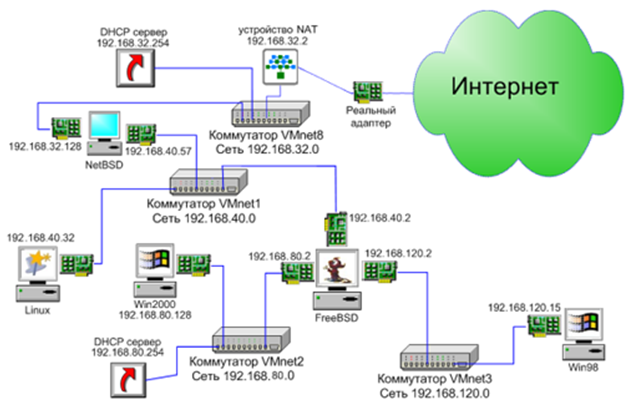
\includegraphics[scale = 0.8]{images/0.png}
	\caption{Архитектура компьютерной сети}
	\label{image:0}
\end{figure}

\section{Виртуальное макетирование сетевой конфигурации}

Конфигурация сегментов сети в соответствии с архитектурой:

\begin{figure}[h!]
	\centering
	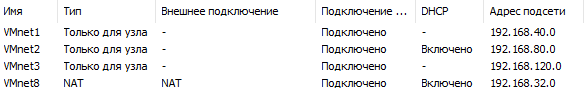
\includegraphics[scale = 1.1]{images/1.png}
	\caption{Настройка сегментов сети в VMware Workstation}
	\label{image:1}
\end{figure}

Для сети VMnet8 было задано перенаправление 80 порта следующим образом:

\begin{figure}[h!]
	\centering
	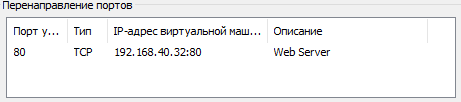
\includegraphics[scale = 1.1]{images/6_1.png}
	\caption{Перенаправление 80 порта для HTTP сервера}
	\label{image:3}
\end{figure}

\section{Виртуальное макетирование хостов}

Для целей лабораторной работы было создано 5 виртуальных машин в соответствии с архитектурой сети (рис. \ref{image:0}):

\begin{itemize}
	\item Windows 98
	\item Windows XP
	\item Ubuntu
	\item FreeBSD
	\item NetBSD
\end{itemize}

Для каждой ОС были добавлены сетевые адаптеры сегментов сети в соответствии с архитектурой сети (рис. \ref{image:0}).

Для чистоты эксперимента встроенные межсетевые экраны в данных ОС были отключены.

\clearpage

\section{Настройка TCP/IP-сети}

\subsection{Windows 98}

Настройка сети для конфигурации IPv4:

\begin{figure}[h!]
	\centering
	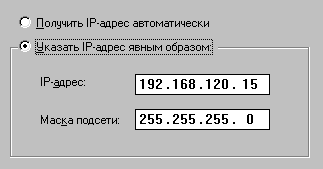
\includegraphics[scale = 0.7]{images/2_1.png}
	\caption{}
	\label{image:4}
\end{figure}

\begin{figure}[h!]
	\centering
	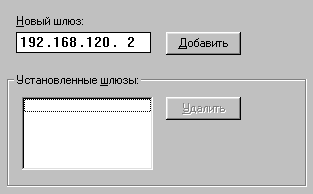
\includegraphics[scale = 0.7]{images/2_2.png}
	\caption{}
	\label{image:5}
\end{figure}

После перезагрузки системы удостоверимся, что конфигурация адаптера сохранилась:

\begin{figure}[h!]
	\centering
	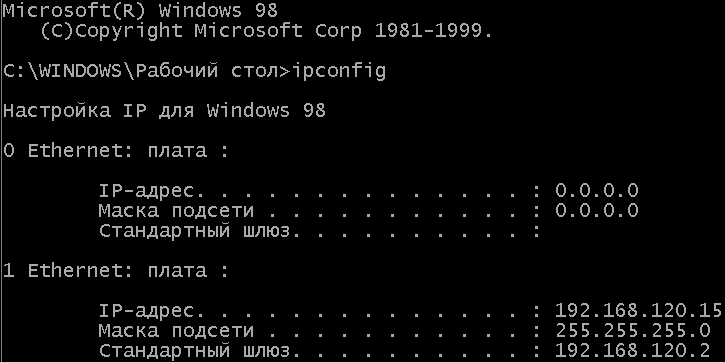
\includegraphics[scale = 0.8]{images/2_3.png}
	\caption{}
	\label{image:6}
\end{figure}

\clearpage

\subsection{Windows XP}

Настройка сети для конфигурации IPv4:

\begin{figure}[h!]
	\centering
	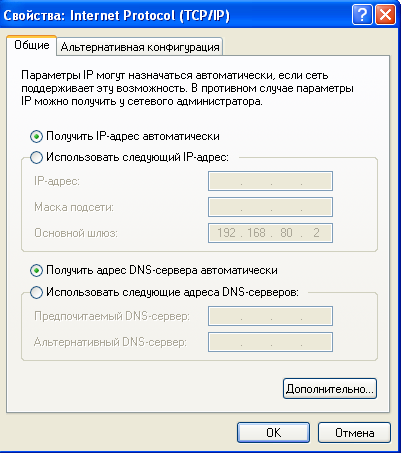
\includegraphics[scale = 1.00]{images/3_1.png}
	\caption{}
	\label{image:7}
\end{figure}

После перезагрузки системы удостоверимся, что конфигурация адаптера сохранилась:

\begin{figure}[h!]
	\centering
	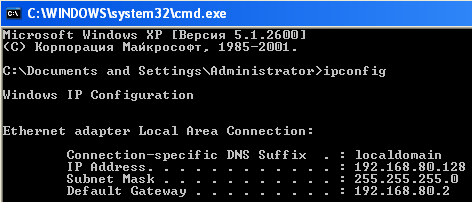
\includegraphics[scale = 0.95]{images/3_2.png}
	\caption{}
	\label{image:8}
\end{figure}

\clearpage

\subsection{Ubuntu}

Настройка сети для конфигурации IPv4:

\begin{figure}[h!]
	\centering
	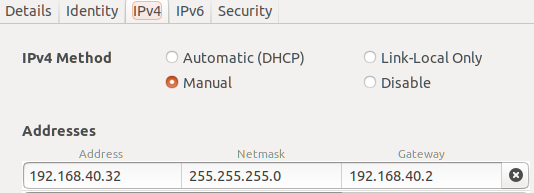
\includegraphics[scale = 0.95]{images/4_1.png}
	\caption{}
	\label{image:9}
\end{figure}

После перезагрузки системы удостоверимся, что конфигурация адаптера сохранилась:

\begin{figure}[h!]
	\centering
	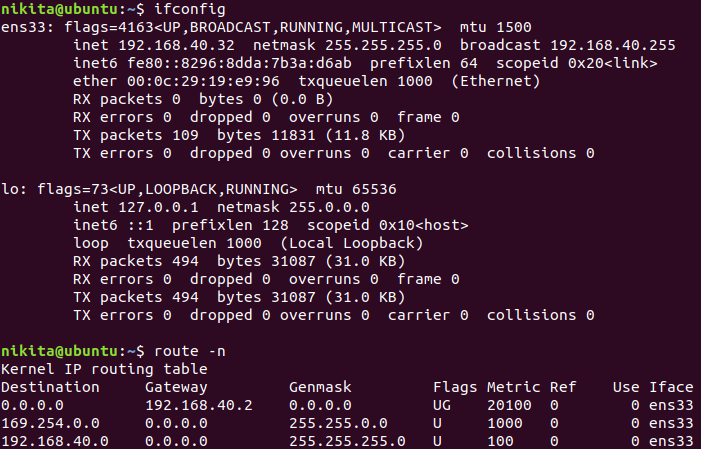
\includegraphics[scale = 0.9]{images/4_2.png}
	\caption{}
	\label{image:10}
\end{figure}

\clearpage

\subsection{FreeBSD}

Настройка сети для конфигурации IPv4:

\begin{figure}[h!]
	\centering
	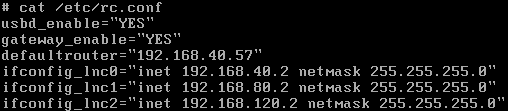
\includegraphics[scale = 1.15]{images/5_1.png}
	\caption{}
	\label{image:11}
\end{figure}

После перезагрузки системы удостоверимся, что конфигурация адаптера сохранилась:

\begin{figure}[h!]
	\centering
	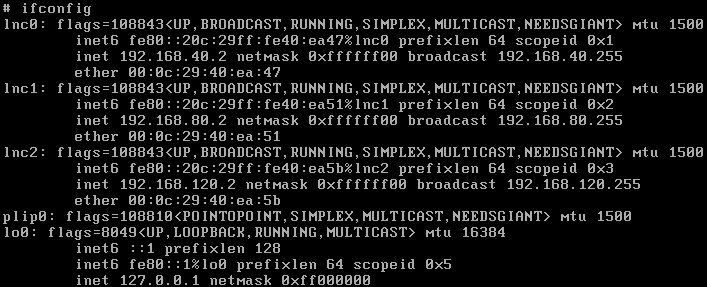
\includegraphics[scale = 0.95]{images/5_2.png}
	\caption{}
	\label{image:12}
\end{figure}

\clearpage

\subsection{NetBSD}

Настройка сети для конфигурации IPv4:

\begin{figure}[h!]
	\centering
	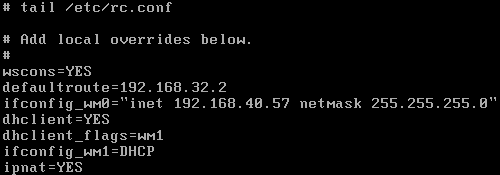
\includegraphics[scale = 1.2]{images/6_2.png}
	\caption{}
	\label{image:13}
\end{figure}

После перезагрузки системы удостоверимся, что конфигурация адаптера сохранилась:

\begin{figure}[h!]
	\centering
	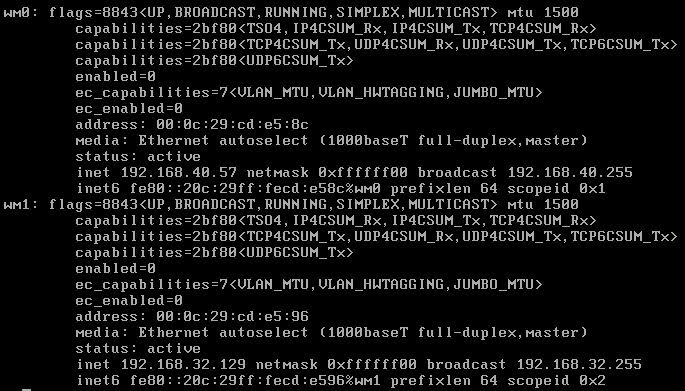
\includegraphics[scale = 0.9]{images/6_3.png}
	\caption{}
	\label{image:14}
\end{figure}

\section{Тестирование TCP/IP-сети}

Для каждого узла сети проверим доступность с помощью утилиты ping:

\begin{itemize}
	\item Шлюза;
	\item Узла NetBSD (192.168.40.57);
	\item Удаленного DNS сервера Google (8.8.8.8);
\end{itemize}

Для каждого узла тестирование прошло успешно, что говорит о правильном проектировании сети.

\section{Вывод}

В данной работе была рассмотрена эмуляция корпоративной компьютерной сети (ККС), которая содержит три основных и один вспомогательный сегмент сети.

Моделирование ККС произведено при помощи средств виртуализации VMWare. Количество сегментов сети ограничивается 20, что вполне достаточно для виртуализации небольших компьютерных сетей, однако, для больших стоит использовать специализированные средства виртуализации.

\end{document}